\documentclass[a4paper, 10pt]{article}
\usepackage{amsmath}
\usepackage{amsthm}
\usepackage{amssymb}	
\usepackage{graphicx}
\usepackage{mathtools}
\usepackage{multirow}
\usepackage{hyperref}
\usepackage{natbib}
\usepackage[utf8]{inputenc}
\usepackage[T1]{fontenc}

\topmargin 0.0cm
\oddsidemargin 0.2cm
\textwidth 16cm  
\textheight 21cm
\footskip 1.0cm
\linespread{1.5}  


% Citation styles
\bibliographystyle{apalike}
\setcitestyle{authoryear, open={(}, close={)}}

\begin{document}
%-------------------------------------------------------------------------------------------------
%--- Title
%-------------------------------------------------------------------------------------------------
\begin{center}
    \Huge
    \textbf{Proto-word reconstruction with NNs}
\end{center}
%-------------------------------------------------------------------------------------------------
%--- Prev work
%-------------------------------------------------------------------------------------------------
\section*{Cognate sets \& proto-words}
\begin{itemize}
    \item Cognate set: N-tuple of related/homologous words in $n$ languages:
    \begin{equation}
        <father,Vater,vader,fa\eth ir>
    \end{equation}
    \item Proto-word: The common ancestor from which the words in the cognate set descend, in (1) from Proto-Germanic \textit{*fad$\bar{e}$r}
\end{itemize}
\section{Work to build on}
\begin{itemize}
    \item \cite{bouchard-Cote_et_al:2013}, phylogenetic inference performed on a large Austronesian dataset (reversible-jump MCMC, so not strictly what we want).
    The goal is to reconstruct a phylogenetic tree, and \cite{bouckaert_et_al:2012}, also inferring geographic diffusion of the IE family.
    \item \cite{ciobanu_ab_2018}, using conditional random fields \& RNNs \cite{ciobanu_ab_2018} to reconstruct Latin words from Romance cognate data.
    \item \cite{meloni_ab_2019} also RNN, pipeline similar to neural machine translation. Inputs are character + language embedding vectors. (Encoder-Decoder)
    \item Cognate identification with siamese CNNs using either string similarity metrics as Levenshtein distance
    \cite{wilding_cross-family_2019} or phonetic feature arrays (multi-hot encodings) \cite{rama_siamese_2016}.
    \begin{figure}[htp]
        \centering
        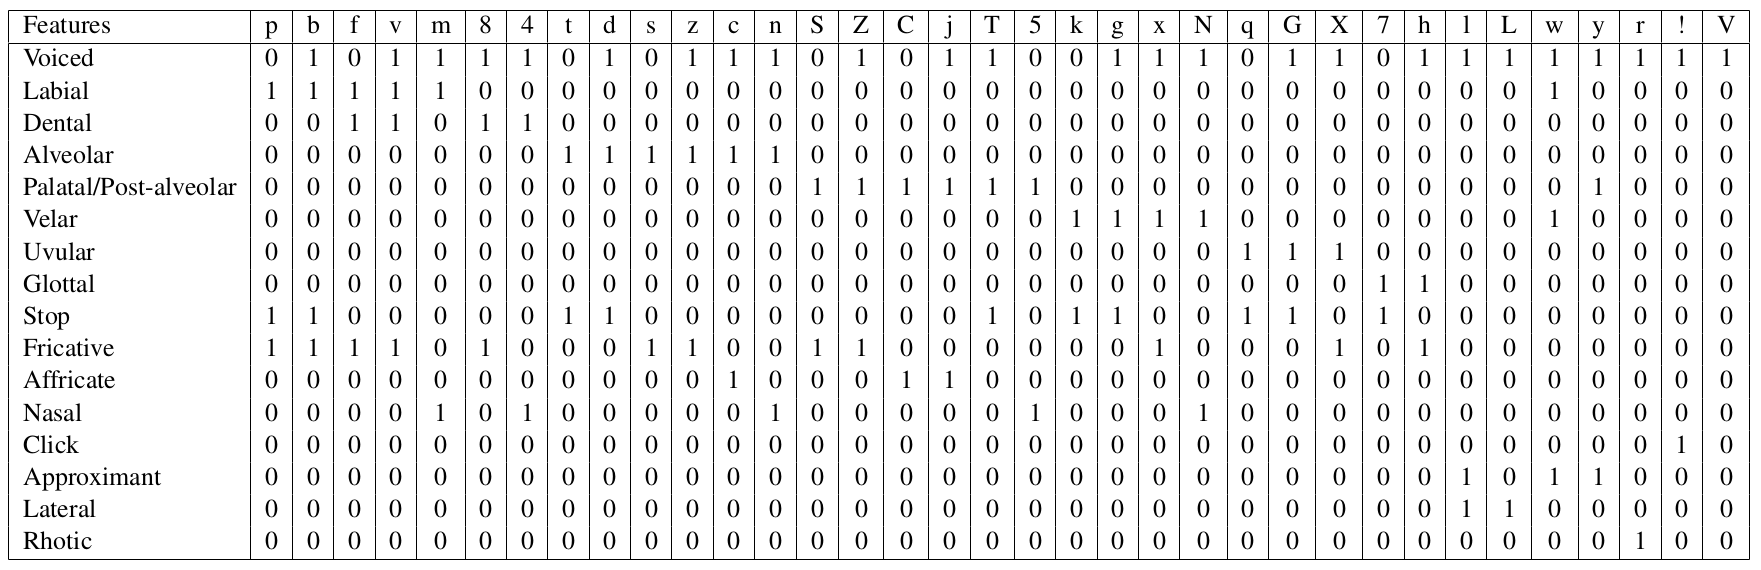
\includegraphics[width=0.85\textwidth]{graphics/rama_PhoneticCNN.png}
        \caption{Phone encodings in \cite{rama_siamese_2016}, p.1021}
        \label{figure:rama_2016}
    \end{figure}
\end{itemize}

%-------------------------------------------------------------------------------------------------
%--- Data
%-------------------------------------------------------------------------------------------------
\newpage
\section{Data sources} 
\begin{itemize}
    \item Wiktionary 
    \begin{itemize}
        \item Many datapoints of dubious quality
        \item Would have to do most of the data extraction ourselves
        \item Data dumps available \href{https://dumps.wikimedia.org/enwiktionary/}{here}
        \item Technically it should be possible possible to get \href{https://wiki.dbpedia.org/wiktionary-rdf-extraction}{RDF data}
    \end{itemize}
    \item \href{http://ielex.mpi.nl/}{Indo-European lexical cognacy database}
    \begin{itemize}
        \item Used by famous \cite{bouckaert_et_al:2012}
        \item No longer maintained (since 2016)
        \item Only Indo-European data, which may be a bit over-investigated
        \item But: plain TSV
    \end{itemize}
    \item \href{https://starling.rinet.ru/downl.php?lan=en}{Evolution of human language project} (used in \cite{hruschka_detecting_2015}).
    provides cognate data for several Eurasian language families (Altaic, Tungusic, Mongolic, Japonic...)
    \begin{itemize}
        \item I didn't know the format (dBase/.dbf), don't know exactly how to use 
        \item Somewhat outdated (2013)
        \item Pro: Many languages from many families
        \item Could try to reconstruct proto-Altaic (which is a deprecated clade) or proto-Transeurasian
    \end{itemize}
\end{itemize}

%-------------------------------------------------------------------------------------------------
%--- Model
%-------------------------------------------------------------------------------------------------
\newpage
\section{Model architecture}
\begin{itemize}
    \item Code letters for phonological features
    \begin{itemize}
        \item Word = $n_{letters} \times n_{features}$ array (following \cite{rama_siamese_2016}). \\
        Example for PGmc \textit{*fad$\bar{e}r$} with ASJP
        \footnote{https://en.wikipedia.org/wiki/Automated\_Similarity\_Judgment\_Program} 
        encodings:
        \newline
        \newline
        $\begin{Bmatrix}
        f & a & d & \bar{e} & r \\
        f & a & 8 & e & r \\
        \end{Bmatrix}$ \\
        \normalsize
        \item The exact coding depends on the orthographical data available, or we have to do the encoding based on what we know about the exact phonetics of the languages.
    \end{itemize}
    \item MT-like pipleine:
    \begin{itemize}
        \item One cognate as input per time step $\rightarrow$ encoder
        \item Decoder produces proto-word candidate
        \item Encoding of the true proto-word as ground truth
        \item Outputs not only probability distribution over a set of phonetic features, but phonetic encodings $\rightarrow$ visualization of errors (not present in the papers I found)
    \end{itemize}
    \item CNN:
    \begin{itemize}
        \item Difficult for me to get the intuition
        \item In a cognate set like
        \item Kernels should concentrate on phonetic features and/or languages most relevant for reconstruction
        \item Architecture could be very flexible
    \end{itemize}
\end{itemize}

%-------------------------------------------------------------------------------------------------
%--- Model
%-------------------------------------------------------------------------------------------------
\newpage
\section{Work split}
\begin{itemize}
    \item[1)] Until next meeting (07.07.2020):
    \begin{itemize}
        \item Decide on language family (should be the one we can get best data for?)
        \item Get a data sample for development (can be small, produced by hand)
        \item Decide on approach (RNN vs. CNN)
    \end{itemize} 
    \item[2)] After project start:
    \begin{itemize}
        \item Decide on default architecture (everybody)
        \item Get training data (about 2-3000 cognate sets would be ideal, alternatively we can use Swadesh lists)
        \item[] $\rightarrow$ We shouldn't have to change the encoding later
        \item Implement the model
        \item Visualization 
    \end{itemize}
\end{itemize}

%-------------------------------------------------------------------------------------------------
%--- Refs
%-------------------------------------------------------------------------------------------------
\newpage
\bibliography{../bib/NLPwithNN.bib}
\end{document}
